% ----------------------------------------------------------------------
% Capa da dissertação de qualificação
%
% A capa deve conter o nome do autor, o título do trabalho, o local e a
% data. Este arquivo utiliza as macros definidas no
% arquivo main.tex para preencher essas informações. 

\begin{titlepage}
  % A capa é contada mas não numerada
  \thispagestyle{empty}
  % A capa é organizada em três seções verticais: (i) o nome da
  % instituição no topo, (ii) o conteúdo principal no centro e
  % (iii) o local e a data no rodapé. Usamos \vfill para distribuir
  % verticalmente o espaço disponível de forma que as seções do
  % topo e do rodapé fiquem aderidas às margens da página.
  {\bfseries
    % Seção superior: nome da universidade e da faculdade. Inicia
    % imediatamente abaixo da margem superior, sem espaço extra.
    {\centering
      {\normalsize \MakeUppercase{Universidade de São Paulo}}\\
      {\normalsize \MakeUppercase{Faculdade de Medicina}}\\
    }\par

    % Espaço vertical até a seção central
    \vfill

    % Seção central: nome do autor, título do trabalho e imagem
    % institucional. As quebras de linha com espaços definem a
    % separação entre os elementos.
    {\centering
      {\normalsize \autor}\\[1.5cm]
      % O título do trabalho pode ocupar mais de uma linha; para manter a
      % mesma entrelinha utilizada no restante do documento (1,5 linhas),
      % \setstretch localmente aplicado. Isso garante que, se o título
      % quebrar em várias linhas, o espaçamento entre elas será de 1,5 linhas.
      {\normalsize\begingroup\setstretch{1.5}\titulo\par\endgroup}
      \vspace{2cm}
      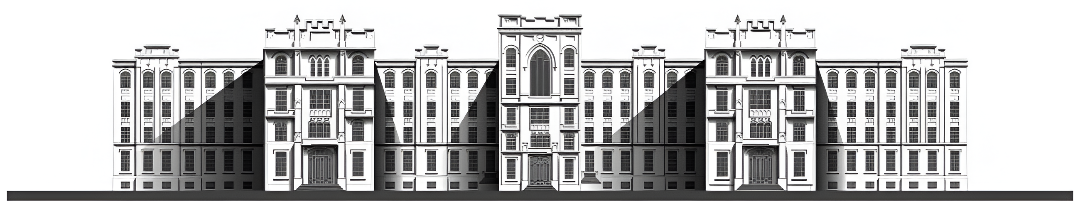
\includegraphics[width=\logowidth]{figuras/instituicao.png}\\
    }\par

    % Espaço vertical até a seção inferior
    \vfill

    % Seção inferior: local e data. Estas linhas aparecem junto à
    % margem inferior, respeitando a mesma fonte e alinhamento central.
    {\centering
      {\normalsize \local}\\
      {\normalsize \datadeposit}\\
    }\par
  }
\end{titlepage}